\documentclass[10pt,twocolumn]{article}
\usepackage[letterpaper,margin=1in]{geometry}
\usepackage{amsmath,amssymb,graphicx,booktabs}
\usepackage[hidelinks]{hyperref}
\usepackage{url}
\usepackage{fontspec}
% Three-glyph subset of Noto Sans CJK SC; see figures/Noto-OFL.txt.
\newfontfamily\authorcjk[Path=figures/]{author-cjk-subset.otf}
\hypersetup{pdfauthor={Guanrong Chen}}
\setlength{\columnsep}{0.23in}
\renewcommand{\topfraction}{0.85}
\renewcommand{\dbltopfraction}{0.85}
\renewcommand{\textfraction}{0.1}
\title{Reference-Guided Style Transfer with a Single LoRA:\\A Diagnostic Study of Texture Generalization}
\author{Guanrong Chen\quad{\authorcjk 陈冠融}\\\small\href{mailto:207878932@qq.com}{207878932@qq.com}}
\date{}

\begin{document}
\maketitle

\begin{abstract}
Reference-guided style transfer must preserve the content of one image while adopting the appearance of another. We examine an Anima-based system that conditions a frozen generator on a content image and a style reference through a single low-rank adapter. Rather than claiming a new state of the art, we reconstruct the implemented training objective and investigate why some references change color or coarse rendering without consistently transferring brushwork. We analyze all 560 LoRA factor tensors, 280 induced update matrices, 138 matched generated images, and 174 controlled single-step forwards. Switching references changes the target hidden state and predicted velocity, establishing a conditional response but not successful disentanglement. An exact spatial-permutation property of the implemented latent Gram statistics yields a counterexample: in one latent-transpose test, relative latent change was 1.16 while the style loss was $5.96\times10^{-14}$. VGG19 and StyleShot-compatible feature probes disagree for particular references. In a subsequent single-case experiment, joint and staged fitting of three reference-derived proxies reduced those proxies but did not visibly reproduce the reference's impasto brushwork. These observations identify measurement and supervision limitations; they establish neither a unique failure mechanism nor a generalization rate.
\end{abstract}

\section{Introduction}
Transferring artistic style from a reference while retaining a separate content image is a conditional generation problem with two competing requirements: the output must preserve the content's structure and respond to the reference's rendering. Classical neural style transfer uses feature correlations as a representation of appearance~\cite{gatys2015}. Recent systems explore style-specific encoders and joint subject--style conditioning~\cite{styleshot2024,uso2025}. These approaches motivate our diagnostics, but we do not compare our system against their reported results under a matched protocol.

Our system keeps an Anima generator frozen~\cite{anima_model_card} and uses one rank-32 LoRA~\cite{lora2021}. Its input contains three token groups: a noisy target, content $B$, and reference $A$. Joint attention allows these groups to exchange information. Separate input slots therefore do not by themselves establish a disentangled representation. The local base file is named \texttt{anima\_baseV10.safetensors}; its exact upstream revision was not independently verified.

This paper makes three limited contributions. First, it documents the actual conditioning and loss operators, including the role of the paired training target. Second, it reports model-level, output-level, and intervention measurements alongside positive and negative visual examples. Third, it exposes a concrete invariance of the style loss and tests reference-derived, jointly or progressively fitted proxies. The findings are diagnostic observations for the investigated checkpoint, not a claim of a novel general-purpose transfer method.

\begin{figure*}[t]
\centering
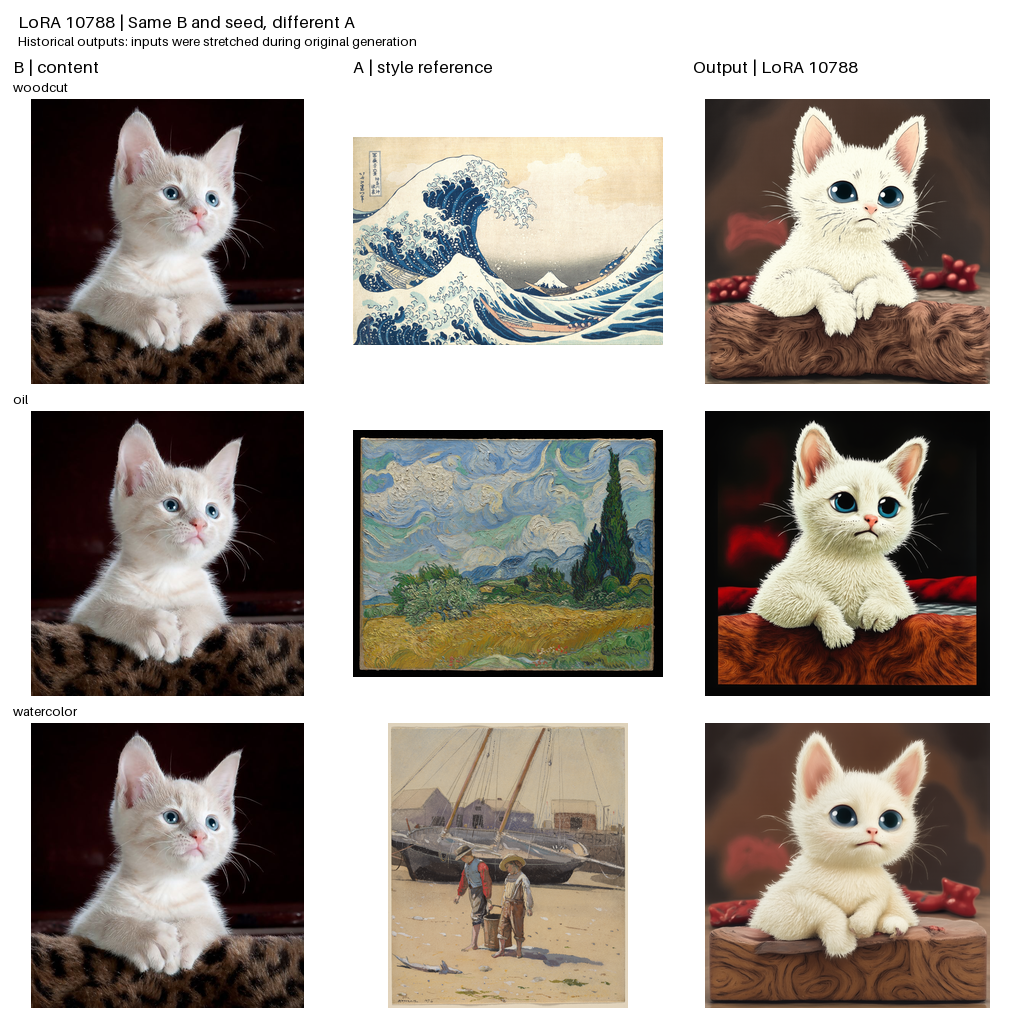
\includegraphics[width=0.85\textwidth]{figures/cats_styles.png}
\caption{Retrospectively selected examples from checkpoint 10788. Columns show content $B$, reference $A$, and output; rows use woodcut, oil, and watercolor references. Rendering changes, but faithful replication of the reference medium is not established. Generation used seed 20261014 and 30 Euler steps. Historical generation inputs were square-stretched; displayed references preserve their aspect ratio.}
\label{fig:examples}
\end{figure*}

\begin{figure}[t]
\centering
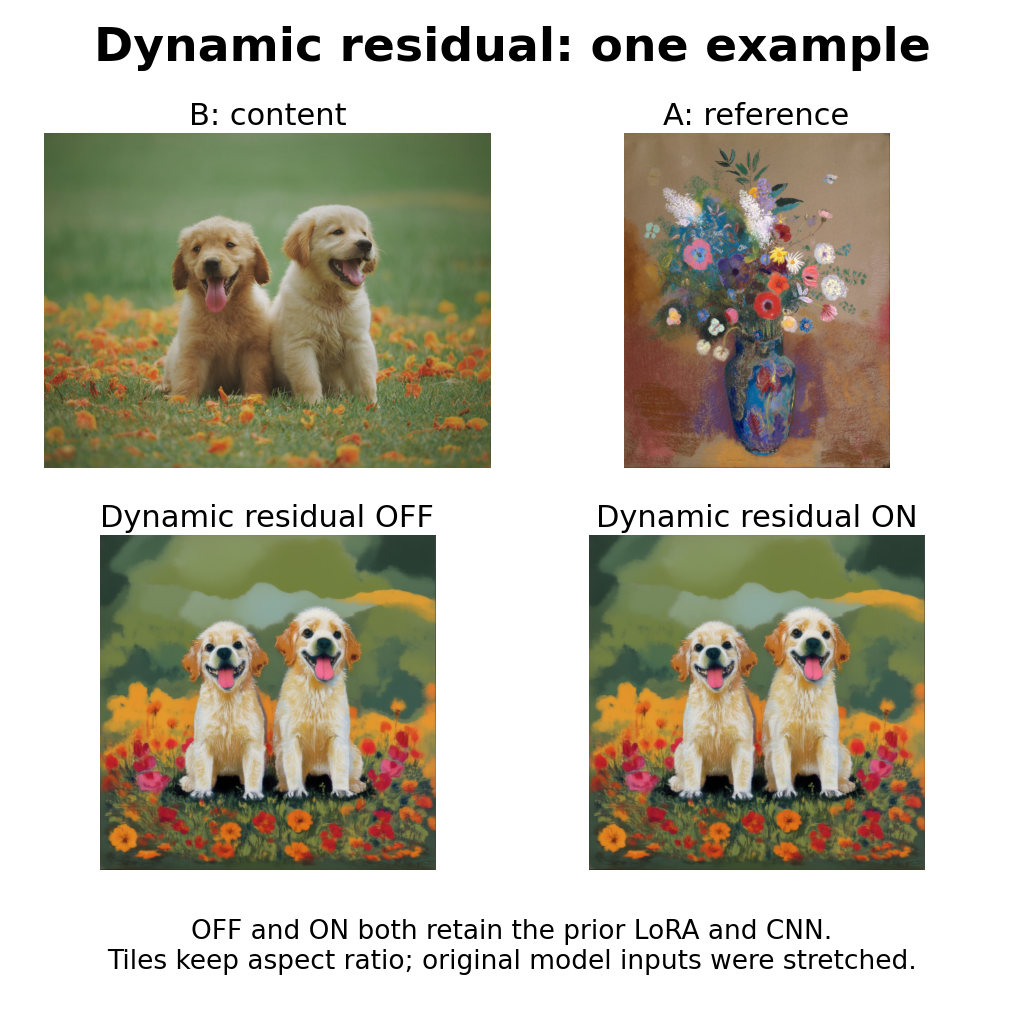
\includegraphics[width=\columnwidth]{figures/dogs_ablation.png}
\caption{A separately trained dynamic residual, retrospectively selected example. The off condition retains LoRA 10135, the old convolutional branch, and reference conditioning. Generation used seed 20261014 and 30 Euler steps; historical inputs were square-stretched.}
\label{fig:dynamic}
\end{figure}

\section{Method}
Figure~\ref{fig:training-route} summarizes the actual training path. It separates the reference condition from the paired target used by the style loss.
\begin{figure*}[t]
\centering
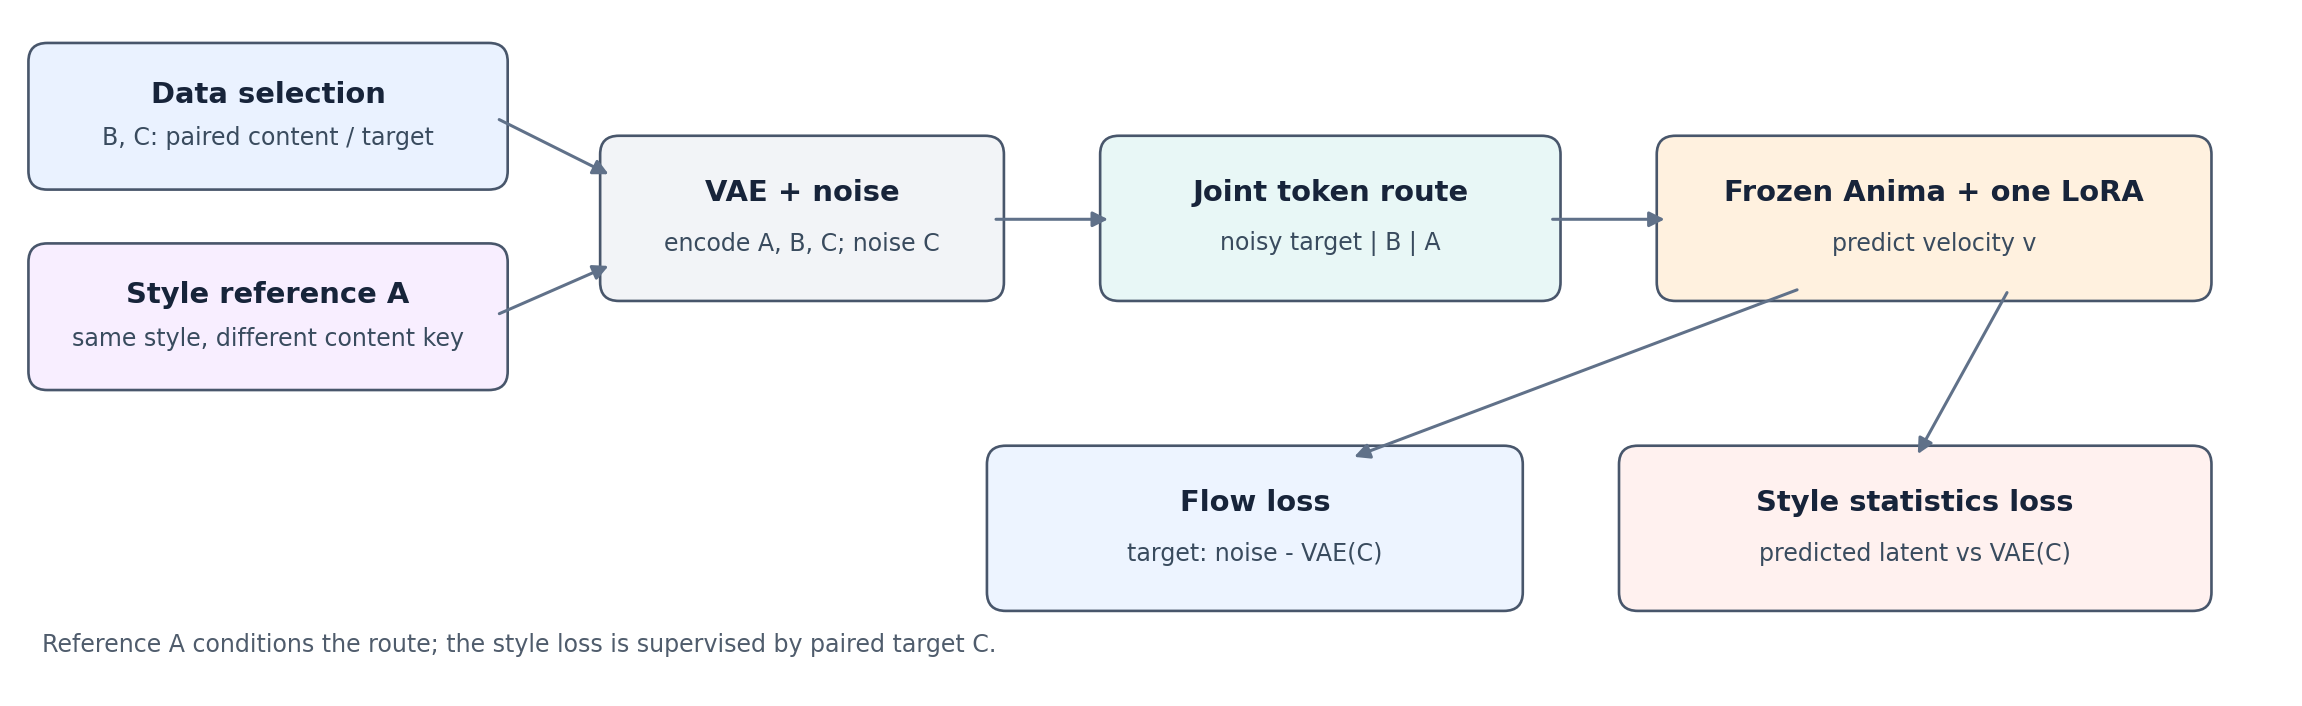
\includegraphics[width=\textwidth]{figures/training_route.png}
\caption{Training path of the audited single-LoRA run. Content $B$, reference $A$, and paired target $C$ are VAE encoded; only $C$ is noised. The joint route feeds the noisy target and both reference latents into Anima. The velocity and style-statistic losses are supervised against $C$; a separate image-space patch loss against $A$ is not present.}
\label{fig:training-route}
\end{figure*}
\subsection{Inputs and flow objective}
Let $B$ denote content, $A$ a reference, and $C$ the paired target used during training. The data loader chooses $A$ from the same style label as $C$, from a different content group, with $A\ne C$; this label rule does not guarantee semantic independence. Let $z_C=E(C)$ be the VAE encoding and $\epsilon\sim\mathcal N(0,I)$. The training code draws $g\sim\mathcal N(0,1)$, $u=\operatorname{sigmoid}(g)$ and $t=3u/(1+2u)$. It forms
\begin{align}
 z_t &= (1-t)z_C+t\epsilon, & v^*&=\epsilon-z_C,\\
 \widehat z_0&=z_t-t\,v_\theta(z_t,t;B,A,\text{text}),\label{eq:zhat}\\
 \mathcal L_{\mathrm{flow}}&=\operatorname{mean}\!\left[(v_\theta-v^*)^2\right].
 \label{eq:flow}
\end{align}
The fixed text instruction requests preservation of the first reference's content and transfer of the second reference's style; it does not name a specific style. At inference the velocity field is integrated over multiple Euler steps before VAE decoding; $\widehat z_0$ in Eq.~\eqref{eq:zhat} is a single-step estimate used during training and, separately, for the inference-time probes described below~\cite{flow2022}.

\subsection{Implemented style operator}
For $s\in\{1,2,4\}$, let $F_s(z)$ denote average-pooled latent features, $N_s$ their spatial count, and $\widetilde F_s$ their channelwise centered features divided by $\sqrt{\operatorname{var}+10^{-6}}$. The normalized channel Gram is
\begin{equation}
 G_s(z)=\widetilde F_s(z)\widetilde F_s(z)^\top/N_s.
 \label{eq:gram}
\end{equation}
With element-averaged smooth $L_1$ distance $\rho$, the implemented style loss is
\begin{align}
 \mathcal L_{\mathrm{style}}
 &= \sum_s w_s\bigl[\rho(G_s(\widehat z_0),G_s(z_C))\nonumber\\
 &\quad+0.25\{\rho(\mu_s(\widehat z_0),\mu_s(z_C))\nonumber\\
 &\qquad\quad+\rho(\sigma_s(\widehat z_0),\sigma_s(z_C))\}\bigr]\nonumber\\
 &\quad+0.10\,\mathcal L_{\mathrm{edge}},
 \quad w=(1,0.7,0.4).
 \label{eq:style}
\end{align}
The edge operator concatenates horizontal and vertical first differences, compares their normalized channel Gram matrices, and adds half the smooth-$L_1$ error of absolute mean, squared mean, and standard deviation. Crucially, Eq.~\eqref{eq:style} compares $\widehat z_0$ with $z_C$: it does not directly align local output patches to $A$.

The total objective is $\mathcal L=\lambda_f\mathcal L_{\mathrm{flow}}+\lambda_s\mathcal L_{\mathrm{style}}$. In the 9999-resume configuration, $\lambda_f=1.25$ and the configured initial $\lambda_s$ was 0.08; after restoring the controller, the first logged value was approximately 0.08087. The value 0.15 was the controller's target weighted style-to-flow gradient-norm ratio, not a fixed style-loss coefficient. Gradients were probed intermittently on sampled rows. Moreover, $\partial\widehat z_0/\partial v_\theta=-tI$ scales the style loss's direct gradient to velocity by $t$, without implying that the full parameter gradient is monotonic in $t$.

\subsection{Adapter and audit quantities}
Each adapted projection computes $Wx+U(Dx)$ with forward scale one. The audited checkpoint has 560 factor tensors (45,875,200 scalar parameters) and 280 induced matrices $\Delta W=UD$, covering ten projections in each of 28 blocks. For singular values $\sigma_i$ of an update, define $q_i=\sigma_i^2/\sum_j\sigma_j^2$ and the entropy effective rank $r_{\rm eff}=\exp(-\sum_iq_i\log q_i)$. Matrix norms and spectra describe parameter structure; they do not directly measure perceptual influence or style quality.

\section{Experimental Protocol}
The training configuration names a local archive \texttt{style\_expert40k.tar}. StyleExpert-40K is described by its authors as a dataset of content, reference, and stylized triplets~\cite{styleexpert2026}; the provenance and exact revision of our local archive were not independently verified. The available 9999-to-10788 training log contains 789 updates and 12,624 row presentations, with 12,624 distinct recorded pair indices, 1,675 content identifiers, 10,890 reference paths, and 140 style labels. No logged row has the same reference and paired-target path. The configured expected 46,046 training pairs is not the number presented during this continuation. The split manifest lists 140/30/37 train/validation/test labels with no exact label overlap; this does not rule out near-duplicate images, related visual styles, or prior exposure in the base model.

\subsection{Data assembly and quality controls}
The source archive was consumed as a pre-existing StyleExpert-style dataset, not a corpus for which this project has a documented human annotation protocol. The parser recognizes source names of the form \texttt{<content>\_src\_<id>} and stylized targets of the form \texttt{extra\_<content>\_<id>\_<style>}. It joins them by content key, uses the suffix as a style label, rejects duplicate member names or ambiguous matches, and records targets without a matching source as orphans. A training row supplies source $B$ and styled target $C$; $A$ is sampled from another row with the same style label and a different content key. These programmatic labels are not evidence of manual image-level annotation or semantic independence.

The recorded label split contains 140/30/37 train/validation/test styles and respectively 46,046/9,766/12,346 raw matched pairs. A 10\% content-key holdout removed 4,533 training-style pairs, leaving a 41,513-pair training pool; the 789 updates presented 12,624 row instances, not the entire pool. Duplicate names and ambiguous joins are checked, and reference/target paths differ in the audited rows. However, the pixel-split routine explicitly reports \texttt{disabled=true}; it did not establish pixel-level or near-duplicate independence. No independent human quality audit, semantic-leakage audit, or per-image licensing review is documented. The archived source tar was later deleted at the owner's request; the \href{https://huggingface.co/datasets/HH-LG/StyleExpert}{official dataset page} is available, but equivalence of a future download to the deleted local revision is unverified. Fixed seeds alone do not reproduce the content split: the code converts a set to a list before seeded shuffling and the original run did not record a fixed \texttt{PYTHONHASHSEED}. Use the retained data plan rather than claiming seed-only reproducibility.

The local archive records 600 outputs from a larger 1,232-output plan; the plan is not treated as completed. The principal balanced subset contains 3 content images, 23 references, and 2 generation seeds, for 138 checkpoint-10788 outputs. A reference label corresponds to one image, and the examples were not reserved as a new sealed benchmark. Repeated content, references, and seeds create correlated observations. The base model's prior exposure to these images and styles is unknown.

For output sensitivity we compute distances between 1,168-dimensional weighted VAE statistics, holding two of $B$, $A$, and seed fixed while changing the third. This descriptor contains Gram, channel-moment, and edge statistics; it is related to the training objective and may encode color, objects, and layout. Its paired distances are descriptive, not style fidelity or disentanglement scores.

We additionally evaluate the 138 outputs against the same 23-reference pool with two auxiliary descriptors. The first averages unit-normalized Gram distances from four local VGG19 feature layers~\cite{vgg2014}. The second uses a locally stored encoder structurally compatible with StyleShot~\cite{styleshot2024} and a custom three-scale cosine score. For each output, the reference advantage is its average distance to the 22 alternatives minus the distance to its matched reference. A positive value means the match is closer than that pool average in the chosen feature space; it is not a success rate. Local weights loaded strictly, but their origin was not independently authenticated.

The VGG probe uses aspect-preserving resize and a 224-pixel center crop; the StyleShot-compatible probe uses a 512-pixel center crop and 8/16/32 patches with a fixed common permutation. The permutation seed is 20261103; the generation seeds are 20261014 and 20261102. Cropping discards some reference margins, whereas historical generation stretched inputs to squares. These protocol differences and the presence of correlated samples limit direct comparison.

We also performed 174 local single-step forwards: $3B\times23A\times2t=138$ external conditions, six author-reference pairs at two $t$ values, and 24 matched controls with LoRA temporarily zeroed in memory. The three-slot route remains present in the zero-LoRA control. The noisy target is anchored to the same cat latent even when $B$ changes, which can put non-cat conditions outside the usual generation distribution. New probe inputs were aspect-preserving and gray-padded. These interventions are not full denoising trajectories.

\begin{figure*}[t]
\centering
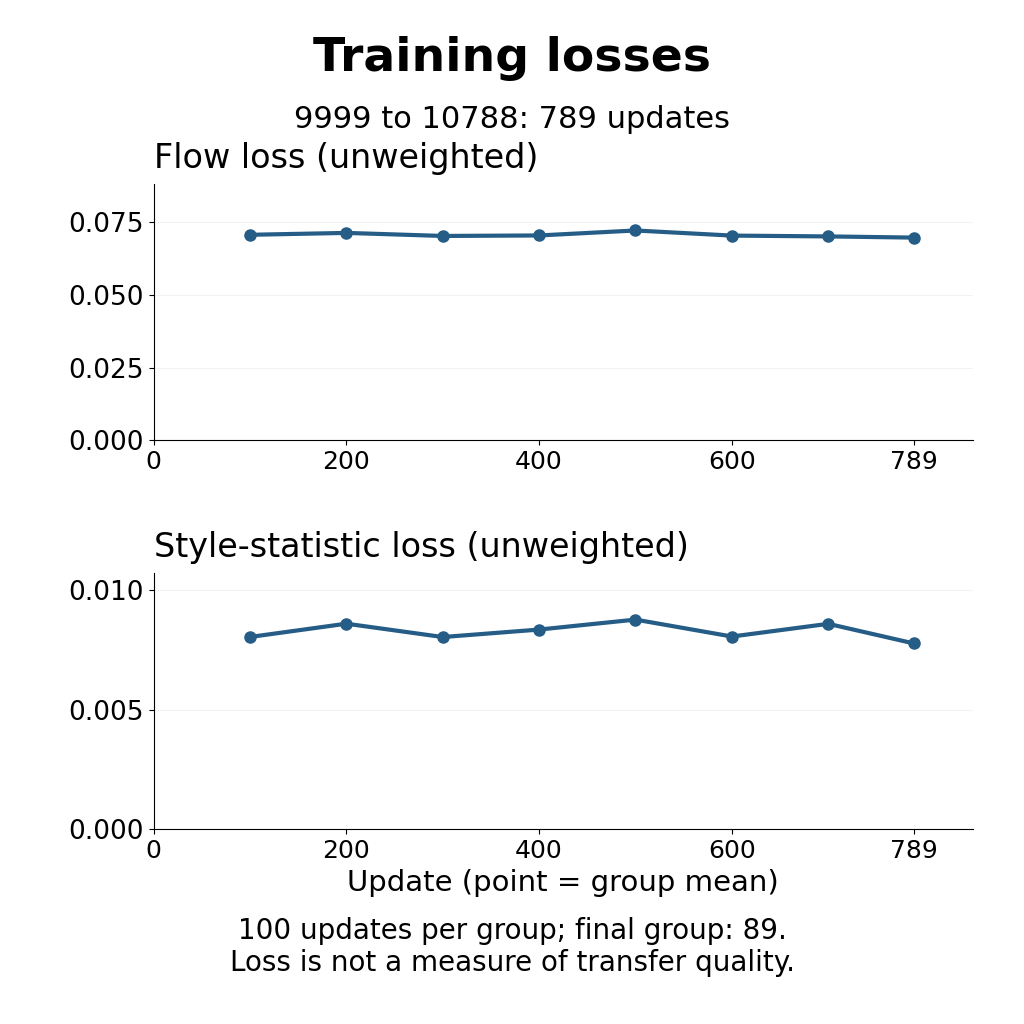
\includegraphics[width=0.47\textwidth]{figures/training.png}\hfill
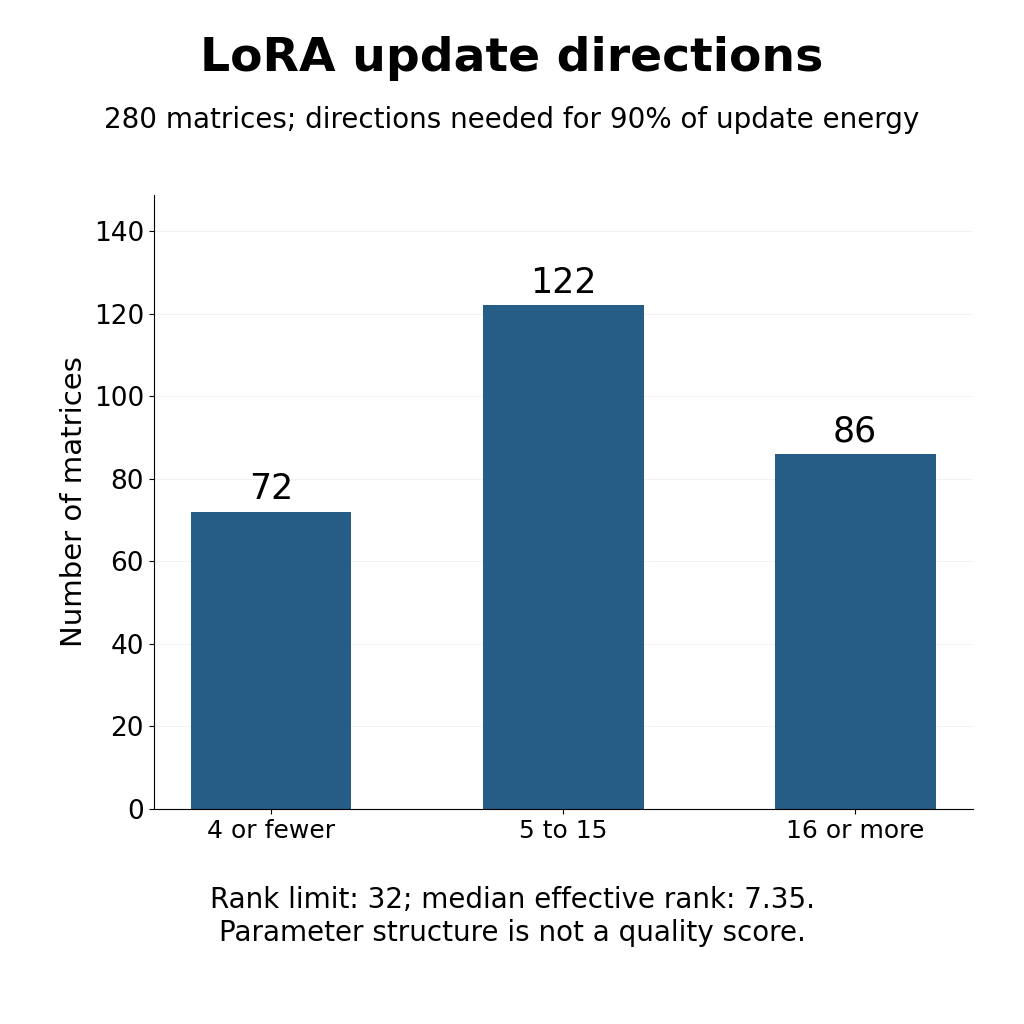
\includegraphics[width=0.47\textwidth]{figures/lora_rank.png}
\caption{Left: 789 logged updates from step 9999 to 10788, averaged in successive windows of 100 updates, except the final window of 89. The two unweighted losses use separate axes and are not perceptual scores. Right: counts of the 280 LoRA update matrices grouped by the number of singular directions needed for 90\% of their energy. Formal rank is at most 32.}
\label{fig:training-rank}
\end{figure*}

\section{Results}
\subsection{Output and proxy behavior}
The median VAE-statistic distance was 0.3469 when swapping $A$ with fixed $B$ and seed (1,518 correlated pairs), 0.7268 when swapping $B$ (138 pairs), and 0.3831 when swapping the seed (69 pairs). The first two changes mix appearance with semantic and spatial differences; stronger sensitivity to $B$ can also reflect the desired preservation of content. These quantities cannot be interpreted as causal contributions or significance tests.

\begin{table}[t]
\centering
\caption{Matched VAE-descriptor output distances. Pair counts are correlated.}
\label{tab:swaps}
\setlength{\tabcolsep}{3pt}
\begin{tabular}{lrrr}
\toprule
Swap & Pairs & Median & P10--P90 \\
\midrule
Reference $A$ & 1518 & 0.347 & 0.172--0.566 \\
Content $B$ & 138 & 0.727 & 0.513--0.875 \\
Seed & 69 & 0.383 & 0.282--0.599 \\
\bottomrule
\end{tabular}
\end{table}

Under the VGG proxy, the per-output reference advantage had median $+0.1007$; it was positive for 115 of 138 outputs, while the matched reference was uniquely nearest in 23 cases. These counts depend on the particular 23-reference pool. Under the StyleShot-compatible proxy, the corresponding per-output cosine advantage had median $+0.0980$. The measures need not agree: for the single cyanotype reference the six-condition median was $-0.1847$ under VGG and $+0.2446$ under the second proxy; for the single watercolor reference it was $+0.1681$ and $-0.0758$, respectively. The models, distances, scales, and crops differ, so the magnitudes cannot be compared across proxies and neither result proves brushstroke fidelity.

A previous image-space optimization illustrates the same measurement risk: for three images, 60 pixel updates reduced a StyleShot-derived distance by approximately 80--87\%, yet the recorded visual review did not pass. Anima and LoRA received zero updates in that test. It is a counterexample for the tested loss and inputs, not a proof that every style encoder fails.

\begin{figure*}[t]
\centering
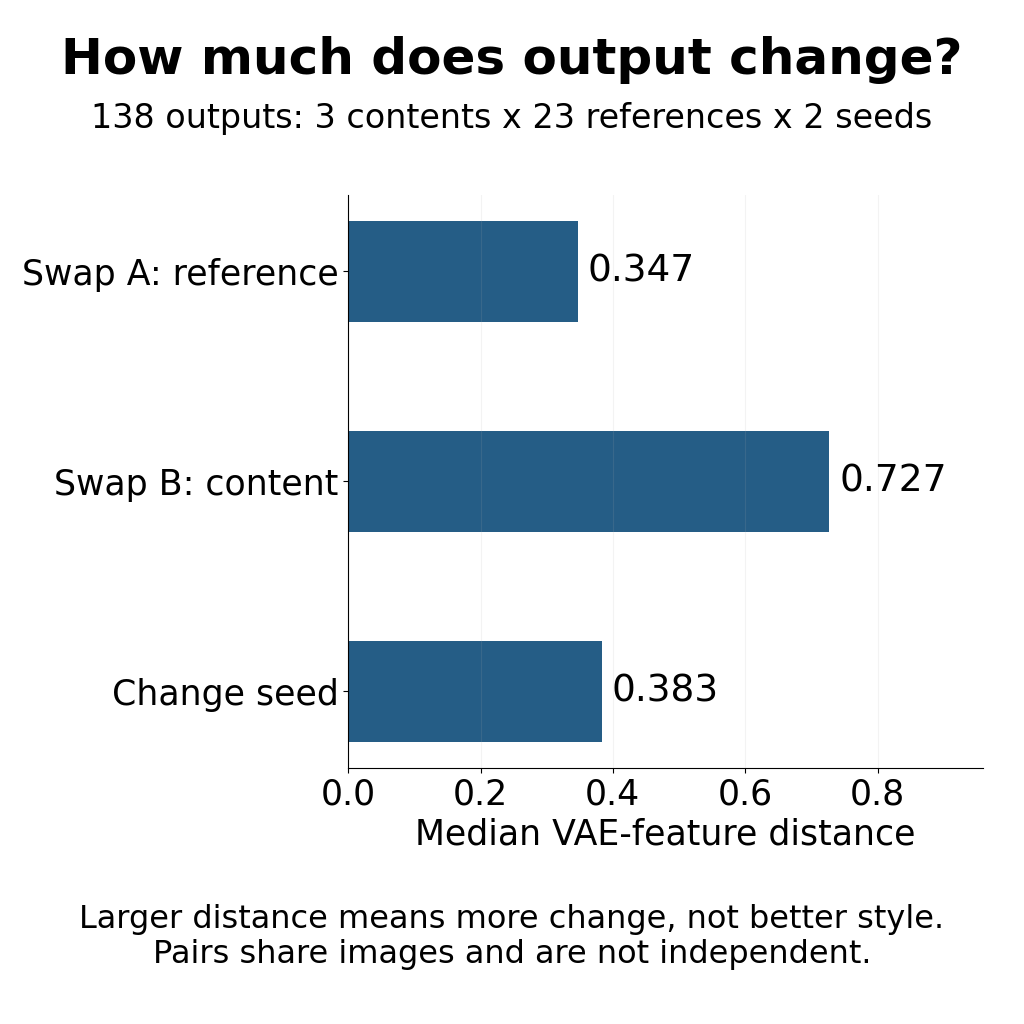
\includegraphics[width=0.47\textwidth]{figures/responses.png}\hfill
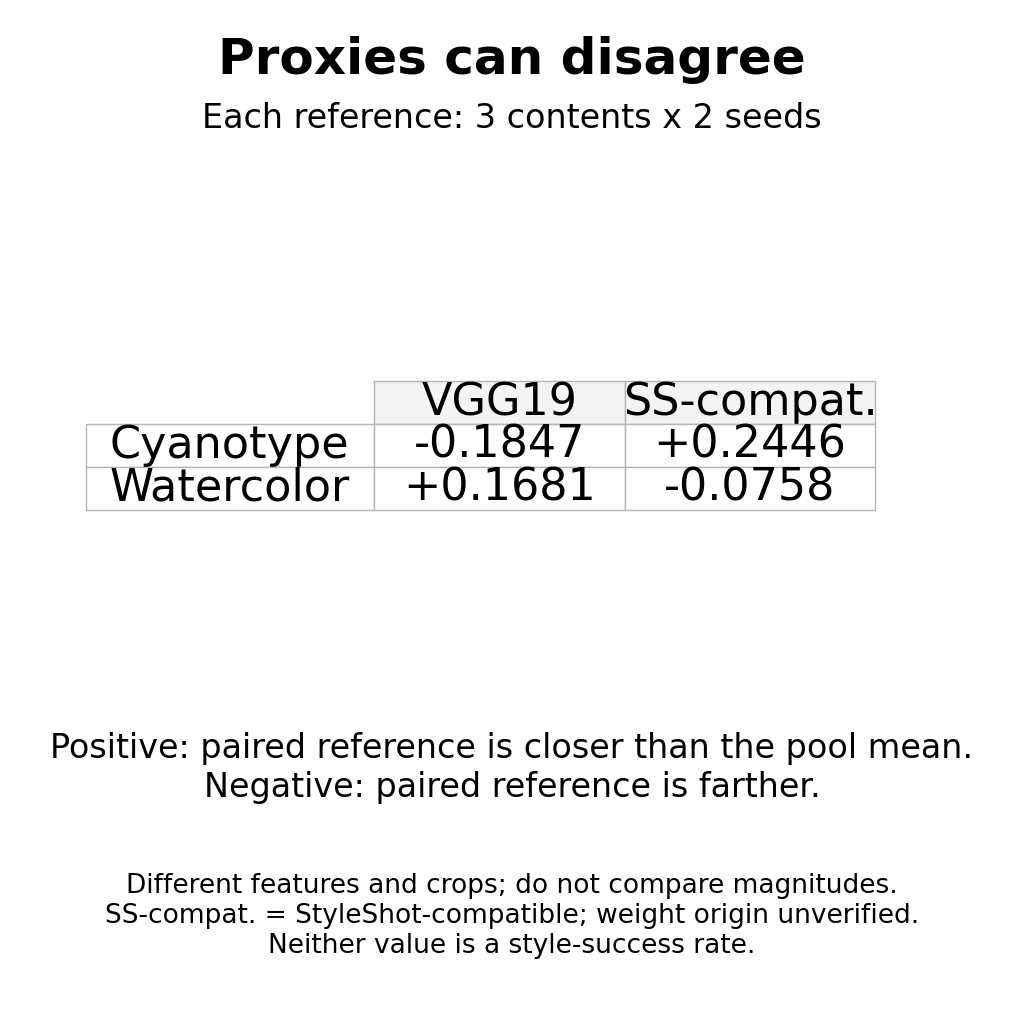
\includegraphics[width=0.47\textwidth]{figures/proxy_disagreement.png}
\caption{Left: median output changes measured by one weighted VAE-statistic descriptor; bigger means more change, not better transfer. Right: reference-advantage medians for two references using a VGG19 Gram proxy and a StyleShot-compatible encoder (SS-compat.; weight origin unverified). Each reference is one image evaluated with three contents and two seeds. The proxies use different distances and crops; signs describe only their respective fixed-pool comparisons.}
\label{fig:outputs}
\end{figure*}

\subsection{Weights and conditional activations}
The median $\lVert\Delta W\rVert_F/\lVert W\rVert_F$ across the 280 adapted projections was 8.25\%, and the median entropy effective rank was 7.35 out of 32. The number of directions needed for 90\% of update energy was at most 4 for 72 projections, 5--15 for 122, and at least 16 for 86. Comparing checkpoints 9999 and 10788, the median relative update change was 15.97\% and the median direction cosine was 0.98765. These are structural statistics, not percentages of generated-image influence; the checkpoints also span different training phases.

The 174 controlled forwards produced $174\times28\times3=14{,}616$ condition--layer--slot groups, each containing 8,388,608 scalar observations. All $122{,}607{,}894{,}528$ observations fell inside the signed-log histogram bins. Only binned summaries were retained. With three contents and four references, the median target-slot response to an $A$ swap at $t=0.35$ was 0.0406, 0.0958, and 0.0228 at blocks 0, 14, and 27, respectively; the final velocity response was 0.0947. Hidden responses were computed after $8\times8$ spatial pooling relative to a reference baseline. Layerwise denominators differ, and self-attention mixes slots; a smaller last-layer ratio does not establish that later layers erased style.

A second, historical $2\times2$ matched intervention fixed $B$, $C$, noise, and $t=0.85$ within each pair. Across two contents and two style labels, wrong-reference minus matched-reference flow MSE was 0.001882, 0.006778, 0.001610, and 0.005724 (Fig.~\ref{fig:condition}). All were positive, supporting conditional influence in these cases, not successful visual transfer.

\begin{figure}[t]
\centering
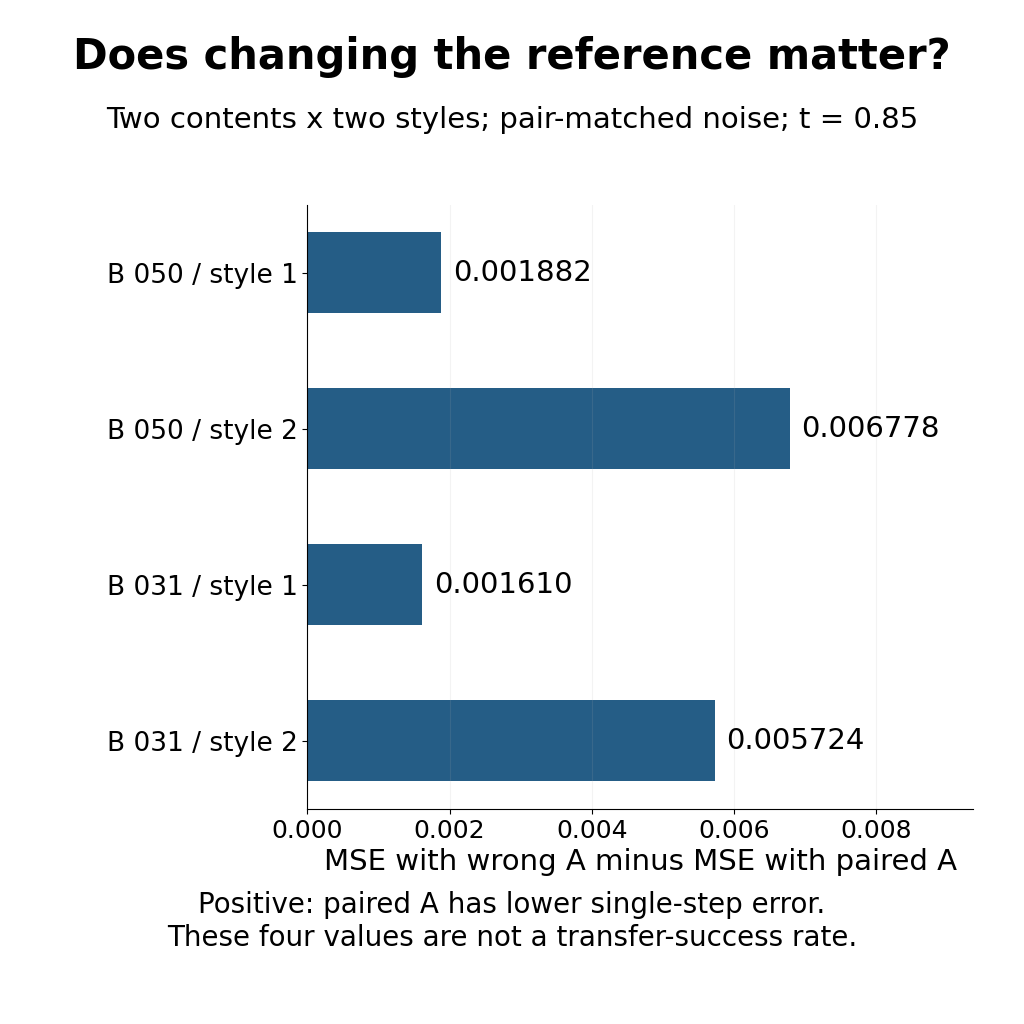
\includegraphics[width=\columnwidth]{figures/condition.png}
\caption{Historical $2\times2$ single-step intervention. Each bar is wrong-reference minus matched-reference flow MSE; style 1 is HeavyMetal and style 2 is geosketch. Positive values indicate lower matched-reference error for these four cases at $t=0.85$, not a transfer success rate.}
\label{fig:condition}
\end{figure}

\subsection{Training and branch trials}
Earlier project records refer to steps 6000, 6280, 7280, and 8280; the available material does not support a causal reconstruction of each stage. The original step-6000 checkpoint was previously reported missing, but its status across all storage locations was not verified. The 9999-resume run was configured for at most 1,000 updates, but the available log ends at local update 789, global step 10788. It used 1024 resolution and effective batch size 16; the recorded LoRA learning rate warmed from $10^{-5}$ to $5\times10^{-5}$. Windowed unweighted flow and style losses showed no clear monotonic decrease (Fig.~\ref{fig:training-rank}); neither loss alone establishes visual improvement.

A separate local-convolution branch received 30 local updates, then 270 additional local updates (300 cumulative), followed by 600 cloud updates (900 cumulative), with the original LoRA frozen. The 600-update record reports 9,600 distinct sampled pairs across 140 style labels. The cloud 0/400/600-update previews (300/700/900 cumulative updates) did not establish stable improvement of external brushwork. Four fixed reference crops covered 25\% of the image area and missed the central $256\times256$ region. One branch output projection had 99.29\% of its energy in four singular directions; this is one projection at one checkpoint, not a statement about all LoRA layers.

A later dynamic residual received 30 local and 100 cloud updates on top of LoRA 10135 and the existing branch. Twelve content/reference pairs were examined with the new residual off and on, using one seed. The recorded review observed some pastel-like edges and ink/paper response, alongside failure to reproduce pointillism or cyanotype and visible content drift. The average on/off RGB absolute change was 0.572 on an 8-bit scale; this is a pixel difference, not a quality score. The test did not establish a stable added visual benefit from the dynamic residual.

Two other pilots each used 15 updates per arm: a reference-ranking term activated on 3 of 15 updates, and a paired-texture condition intervened at three endpoint updates. Their small historical previews did not establish a reliable improvement. Neither pilot is sufficient to reject its entire method class.

\subsection{Reference components and staged inference}
To test a decomposition hypothesis, we construct three reference-derived targets from one oil-painting image $A$: a 16-bin per-channel RGB histogram; grayscale VGG19 feature variation across four directions and two offsets; and symmetric nearest-neighbor distances between spatially pooled grayscale VGG19 patch features. Each representation uses four $224\times224$ crops within the valid image region. These are coupled proxies: direction also responds to object contours, while local features can reflect content and color-derived luminance. They are not learned or verified independent style atoms. Prior work has studied decomposed style features~\cite{styledecomp2018} and compositional diffusion factors~\cite{decompdiff2024}; neither establishes that our existing adapter learns such a basis.

We use the same city content $B$, oil-painting reference $A$, generation seed, checkpoint, prompt, 1024-pixel aspect-preserving gray padding, and 30 Euler updates for both paths. For each image-token LoRA module, an $A$-versus-blurred-$A$ activation probe selects eight spectral directions from $\Delta W_\ell$; the remaining directions form a complementary part. The blurred image is used only for the probe. Every generation update still receives the original $A$. For the 224 image-token modules, candidates alter the native update in memory as
\begin{equation}
\Delta W_\ell(\alpha,\beta)=\Delta W_\ell+\alpha\Delta W_{\ell,S}+\beta\Delta W_{\ell,R}.
\label{eq:parts}
\end{equation}
The text key/value projections remain unchanged. The two spectral groups are not assigned independent style semantics. At solver indices 15, 21, and 27 ($t=0.75,0.5625,0.25$), each path evaluates the same four coefficient pairs: $(0,0)$, $(0.35,0)$, $(0,0.35)$, and $(0.35,0.35)$. For each candidate we decode the one-step estimate in Eq.~\eqref{eq:zhat}, evaluate all three reference proxies, and require the candidate's coarse $B$-latent error to be at most 1.05 times the native candidate's error plus $10^{-8}$. Proxy changes are normalized by the native candidate at that same state, with a $10^{-6}$ floor. The joint path averages all three normalized changes at each decision. The staged path averages the first one, first two, and then all three, retaining earlier objectives. The selected coefficients persist until the next decision.

Each path executes 30 sampler updates, nine additional candidate forwards, one additional blurred-reference probe, and twelve candidate VAE decodes. Their computed budget is matched to each other; the earlier unmodified baseline is cheaper. The paths selected exactly the same spectral sets in all 224 image-token modules during the probe. Intermediate panels are estimates of $\widehat z_0$, not completed half-trajectory images. The experiment involves one $A$, one $B$, one seed, and no parameter updates.

\begin{table}[t]
\centering
\caption{Final reference-proxy errors for the single oil/city case; lower is closer only under each proxy. They are not perceptual success rates.}
\label{tab:parts}
\setlength{\tabcolsep}{3pt}
\begin{tabular}{lrrr}
\toprule
Path & Color & Direction & Texture \\
\midrule
Native & 0.04381 & 0.01173 & 0.11174 \\
Joint & 0.04234 & 0.00979 & 0.10036 \\
Staged & 0.04321 & 0.01055 & 0.10407 \\
\bottomrule
\end{tabular}
\end{table}

\begin{figure*}[t]
\centering
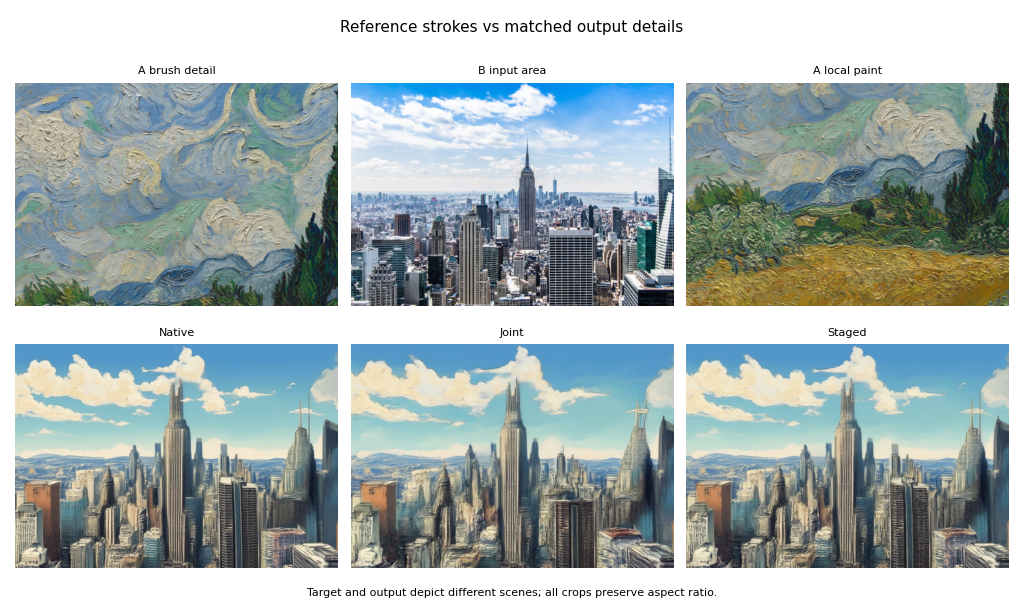
\includegraphics[width=0.9\textwidth]{figures/a_parts_detail.png}
\caption{Single-case reference-decomposition experiment: oil reference details, city content, and matched native/joint/staged output crops. All generation outputs are 1024-pixel square with aspect-preserving padding. Both fitted paths preserve the broad skyline but redraw details and fail to reproduce the reference's raised, curved brushwork. Reference and output crops show different subjects; color, directional, and VGG proxies cannot independently establish faithful brush transfer.}
\label{fig:parts}
\end{figure*}

The joint path selected $(0.35,0.35)$ at all three decisions; the staged path selected $(0,0)$, then $(0.35,0.35)$ twice. In exact arithmetic, equal additions to complementary spectral parts scale the image-token LoRA update by 1.35; BF16 evaluation introduces rounding differences. Thus the observed path difference is largely the onset time of this near-uniform increase, not evidence that three components were separately reconstructed. Although all three final proxies decreased relative to the saved native image (Table~\ref{tab:parts}), visual inspection did not find the target's impasto or curved strokes (Fig.~\ref{fig:parts}). All candidates passed the coarse content guard at the recorded decision points, which does not guarantee final content preservation.

At the first decision, the two individual $+0.35$ interventions changed the three proxies, relative to the native candidate, by $(+0.614,-10.980,-5.991)\%$ and $(+0.441,-4.867,-1.908)\%$. Their three-dimensional finite-response cosine is 0.9915 under this normalization, indicating nearly aligned responses in these proxies at this state and perturbation size. At the joint path's third decision it is approximately 0.747. These finite perturbations are neither an exact full-model Jacobian nor proof that the LoRA's global style space is one-dimensional.

\section{Operator Analysis}
\subsection{A concrete invariance}
For a flattened feature matrix $F\in\mathbb R^{C\times N}$ and spatial permutation matrix $P$, channel statistics are permutation invariant and $\widetilde{FP}=\widetilde F P$. Therefore,
\begin{equation}
 G(FP)=\frac{\widetilde FPP^\top\widetilde F^\top}{N}=G(F).
 \label{eq:permutation}
\end{equation}
In the measured square-latent transpose case, the tested pooling scales commute with transposition and the concatenated horizontal/vertical edge statistics are also rearranged without changing their aggregate. The relative RMS change of the latent was 1.16, whereas the implemented style loss between it and its transpose was $5.96\times10^{-14}$. This demonstrates a specific invariance. A latent transpose is not a rotation of a real image, spatial invariance can be intentional, and the flow loss need not share it. Consequently this observation does not establish the unique cause of failed texture transfer.

A simple reference-cache implementation yielded relative RMS differences of approximately 0.00826--0.01071 from full forward evaluation. In one fixed-state test, directly adding a high-frequency component to the reference velocity difference increased flow MSE at all three sampled $t$ values. These results reject the tested implementations under their tested conditions; they do not rule out all caching or high-frequency methods.

\subsection{Prior Reference Adapters}
The public Anima reference adapter is designed mainly to preserve a character and some appearance from one reference while a prompt changes the scene. Its authors also report weak style-slot behavior in their particular two-slot and style-only experiments~\cite{animaadapter2026}. Our task instead uses separate content and style images. Six aspect-preserving runs used cropped images from the adapter's showcase as references, but we did not rerun that adapter on matched inputs. USO explicitly studies joint subject/style conditioning with alignment and disentanglement objectives~\cite{uso2025}; its reported results are not a matched baseline for our experiments. No superiority claim follows from these comparisons.

\section{Limitations and Conclusion}
The evidence supports a conditional response to $A$ and some qualitative stylistic changes. It also shows recurring failures to reproduce specific texture or medium properties, content drift, and disagreement among proxy metrics. In the single reference-decomposition case, the joint and staged procedures chose largely uniform LoRA increases; neither visually recovered the reference brushwork. This result does not rule out learned style factors or other decomposition mechanisms. The historical outputs used square-stretched inputs; other probes used padding or center crops. The 138-image analysis shares references and contents, uses only two generation seeds, and was conducted after earlier inspection. The archive does not contain a completed 1,232-image evaluation, a sealed test, a blinded human study, or a fair external-model rerun. Pretraining exposure to the evaluation images is unknown. Two upsampled references had VAE reconstruction PSNR of 39.51 and 35.91 dB in their valid regions; this does not exclude lost high-frequency detail in other images.

A useful next experiment should first test whether a proposed local descriptor ranks same-style/different-content patches closer than same-content/different-style patches. With that behavior established, matched single-LoRA training arms should be evaluated using fixed inputs, seeds, full-resolution crops, and a separately held-out assessment. The present evidence is insufficient to select a larger rank, a higher style coefficient, or more training steps as a stand-alone remedy.

\section*{Data and code availability}
Selected source code, the ComfyUI node and workflow, experiment records, and research figures are available in the \href{https://github.com/lightlanguage1/anima-single-lora-style-transfer}{project repository}. The 10788 LoRA checkpoint and its applicable license notices are available on \href{https://huggingface.co/lightlanguang/Anima-Single-LoRA-Style-Transfer-10788}{Hugging Face}. The local evidence index also records the 600 archived output records, operator analyses, and reference-decomposition pilots; the complete local archive has not been publicly deposited. The original training archive was deleted, its exact upstream revision is unverified, and full independent reproduction has not been established. Rights for individual source images require review before reuse.

\section*{Image sources}
The cat photograph is credited to Pixabay / Pexels (\href{https://www.pexels.com/photo/white-and-grey-kitten-on-brown-and-black-leopard-print-textile-45201/}{image 45201}); the dogs photograph is from \href{https://www.pexels.com/photo/1108099/}{Pexels 1108099}; the city photograph is credited to Lukas Kloeppel / \href{https://www.pexels.com/photo/empire-state-building-new-york-466685/}{Pexels 466685}. The pictured art references are Hokusai, \emph{Under the Wave off Kanagawa} (The Met \href{https://www.metmuseum.org/art/collection/search/45434}{45434}); van Gogh, \emph{Wheat Field with Cypresses} (\href{https://www.metmuseum.org/art/collection/search/436535}{436535}); Homer, \emph{A Basket of Clams} (\href{https://www.metmuseum.org/art/collection/search/12388}{12388}); and Redon, \emph{Bouquet of Flowers} (\href{https://www.metmuseum.org/art/collection/search/437379}{437379}). The Met identifies all four cited works as public domain. The pictured sources visually match the cited pages; visual matching does not establish the exact historical downloaded files or clear all reuse rights.

\begin{thebibliography}{11}
\bibitem{gatys2015} L.~A.~Gatys, A.~S.~Ecker, and M.~Bethge. A neural algorithm of artistic style. \href{https://arxiv.org/abs/1508.06576}{arXiv:1508.06576}, 2015.
\bibitem{lora2021} E.~J.~Hu et al. LoRA: Low-rank adaptation of large language models. \href{https://arxiv.org/abs/2106.09685}{arXiv:2106.09685}, 2021.
\bibitem{flow2022} Y.~Lipman, R.~T.~Q.~Chen, H.~Ben-Hamu, M.~Nickel, and M.~Le. Flow matching for generative modeling. \href{https://arxiv.org/abs/2210.02747}{arXiv:2210.02747}, 2022.
\bibitem{vgg2014} K.~Simonyan and A.~Zisserman. Very deep convolutional networks for large-scale image recognition. \href{https://arxiv.org/abs/1409.1556}{arXiv:1409.1556}, 2014.
\bibitem{styleshot2024} J.~Gao et al. StyleShot: A snapshot on any style. \href{https://arxiv.org/abs/2407.01414}{arXiv:2407.01414}, 2024.
\bibitem{uso2025} S.~Wu et al. USO: Unified style and subject-driven generation via disentangled and reward learning. \href{https://arxiv.org/abs/2508.18966}{arXiv:2508.18966}, 2025.
\bibitem{animaadapter2026} ElectronGirl. Anima reference adapter research: Experiment log. 2026. \url{https://github.com/ElectronGirl/anima-ref-adapter-research/blob/main/docs/experiments.md}.
\bibitem{styledecomp2018} M.~Li, S.~Tu, and L.~Xu. Computational decomposition of style for controllable and enhanced style transfer. \href{https://arxiv.org/abs/1811.08668}{arXiv:1811.08668}, 2018.
\bibitem{decompdiff2024} J.~Su, N.~Liu, Y.~Wang, J.~B.~Tenenbaum, and Y.~Du. Compositional image decomposition with diffusion models. ICML, 2024. \href{https://arxiv.org/abs/2406.19298}{arXiv:2406.19298}.
\bibitem{anima_model_card} CircleStone Labs and Comfy Org. Anima model card. \url{https://huggingface.co/circlestone-labs/Anima}.
\bibitem{styleexpert2026} S.~Zhu et al. Mixture of style experts for diverse image stylization. \href{https://arxiv.org/abs/2603.16649}{arXiv:2603.16649}, 2026. Dataset: \href{https://huggingface.co/datasets/HH-LG/StyleExpert}{HH-LG/StyleExpert}.
\end{thebibliography}

\appendix
\section{Training, Hardware, and Model-File Identification}
\subsection{Recorded implementation and environment}
The examined continuation used one GPU: the saved preflight report names an NVIDIA RTX 6000D with 83.05 GiB visible memory, PyTorch 2.12.0+cu130, and CUDA 13.0. CPU model, operating-system version, driver version, and a reproducible image digest were not recorded in the available run evidence; they are not inferred from a different instance. Training used resolution 1024, rank 32, BF16 model computation and FP32 LoRA weights, microbatch 1 and effective batch 16 with 16 accumulated model rows. AdamW used $(\beta_1,\beta_2)=(0.9,0.999)$, $\epsilon=10^{-8}$, zero weight decay, and gradient norm clipping at 1. The learning rate was initialized at $10^{-5}$ and linearly warmed to $5\times10^{-5}$ over 100 updates, then held constant in the configured phase. The configuration requested at most 1,000 updates, previews every 100 and checkpoints every 200; the retained log contains 789 updates. A 60 GiB RAM-cache limit, no disk latent cache and seven activation-checkpointed blocks were recorded; these are configuration facts rather than minimum hardware requirements.

\subsection{Training pseudocode}
The following summarizes the audited implementation, not a claim that an isolated package currently reproduces the original environment. The model reads $A$, while the style statistics target $C$.
\begin{verbatim}
for each optimizer update:
  zero accumulated LoRA gradients
  weight_used = controller.weight
  for each of 16 sampled rows:
    B, C, style = paired_record()
    A = same_style_other_content(style)
    zC = VAE(C); e = Gaussian_noise()
    t = shifted_sigmoid_normal()
    zt = (1-t)*zC + t*e
    v = model(zt, t, VAE(B), VAE(A), text)
    zhat = zt - t*v
    accumulate_gradients(
      (1.25*flow(v, e-zC)
      + weight_used*stats(zhat, zC))/16)
  if scheduled_audit:
    update_controller_for_next_step()
  clip_gradient_norm(1); AdamW_step()
  record_metrics_and_scheduled_outputs()
\end{verbatim}
The style controller probes four sampled rows every 32 updates, with target weighted style-to-flow gradient-norm ratio 0.15 and an EMA coefficient 0.9; it restores controller state on resume. Those sparse measurements are not per-update measurements. See Eq.~\eqref{eq:style} for the actual multi-scale statistics and gradient limitation.

\subsection{SHA-256 of available local model files}
Table~\ref{tab:model-digests} lists complete SHA-256 digests measured on the currently available local files on 7 November 2026. These identify the bytes of those files; the 10788 training contract recorded the base/VAE digests as disabled, so the table does not by itself establish their identity to the files loaded in that run. The LoRA is this project's checkpoint, not an upstream base model. The VGG19 and StyleShot-compatible probe weights' exact local origin or file identity was not established here; no digest is asserted for them. Tokenizer revisions and the deleted dataset archive digest are likewise unavailable. The official Anima model card and StyleExpert dataset page provide upstream access and licensing; local filenames alone do not prove upstream revision.
\begin{table}[t]
\centering
\caption{SHA-256 identifiers measured on available local files; not asserted as the missing 10788 training-time digests. Each digest continues on the next line.}
\label{tab:model-digests}
\footnotesize
\setlength{\tabcolsep}{0pt}
\begin{tabular}{l}
\toprule
Local file; SHA-256 on the following line \\
\midrule
\texttt{anima\_baseV10.safetensors} \\
\texttt{bd43b7cffe1ed1153d9c41e7beb2f18c} \\
\texttt{b1273eafbaa3af3edd6a173dc90a006e} \\
\texttt{qwen\_image\_vae.safetensors} \\
\texttt{a70580f0213e67967ee9c95f05bb400e} \\
\texttt{8fb08307e017a924bf3441223e023d1f} \\
\texttt{qwen\_3\_06b\_base.safetensors} \\
\texttt{cd2a512003e2f9f3cd3c32a9c3573f82} \\
\texttt{0bb28c940f73c57b1ddaa983d9223eba} \\
\texttt{lora84\_010788.safetensors} \\
\texttt{20ab06331e98cc99d02132a84dbb20c9} \\
\texttt{570c0499bb603ea669a42aa289a7fa24} \\
\bottomrule
\end{tabular}
\end{table}


\section{Experiment Inventory}
Table~\ref{tab:inventory} separates archived results from planned evaluations. The local evidence index supplies record-level paths and sample definitions; the material is not yet an independently reproducible public release.
\begin{table}[h]
\centering
\caption{Available experiment scopes, not independent estimates of performance.}
\label{tab:inventory}
\setlength{\tabcolsep}{3pt}
\begin{tabular}{lr}
\toprule
Evidence & Scope \\
\midrule
9999 resume & 789 updates \\
Comprehensive archive & 600 / 1,232 planned \\
10788 matched outputs & 138 images \\
Controlled forward probes & 174 forwards \\
Dynamic residual ON/OFF & 12 pairs, 1 seed \\
External reference paths & 4 paths, 1 case \\
Internal spectral paths & 6 paths, 1 case \\
Feedback / uniform control & 2 paths, 1 case \\
Joint/staged A proxies & 2 paths, 1 case \\
\bottomrule
\end{tabular}
\end{table}

\section{Full Distributions}
\label{sec:full_distributions}
Figures~\ref{fig:full-distributions} and~\ref{fig:activation-distributions} present the full $28\times10$ array of adapted-matrix norm ratios and the signed-log hidden-value histograms. Each noise-time panel in the latter figure aggregates the 69 external conditions with active LoRA; author-reference and zero-LoRA controls are not included in that displayed aggregation. The full archived histograms cover all 174 conditions. These views describe the measured parameters and states, not a universal style distribution.
\begin{figure*}[t]
\centering
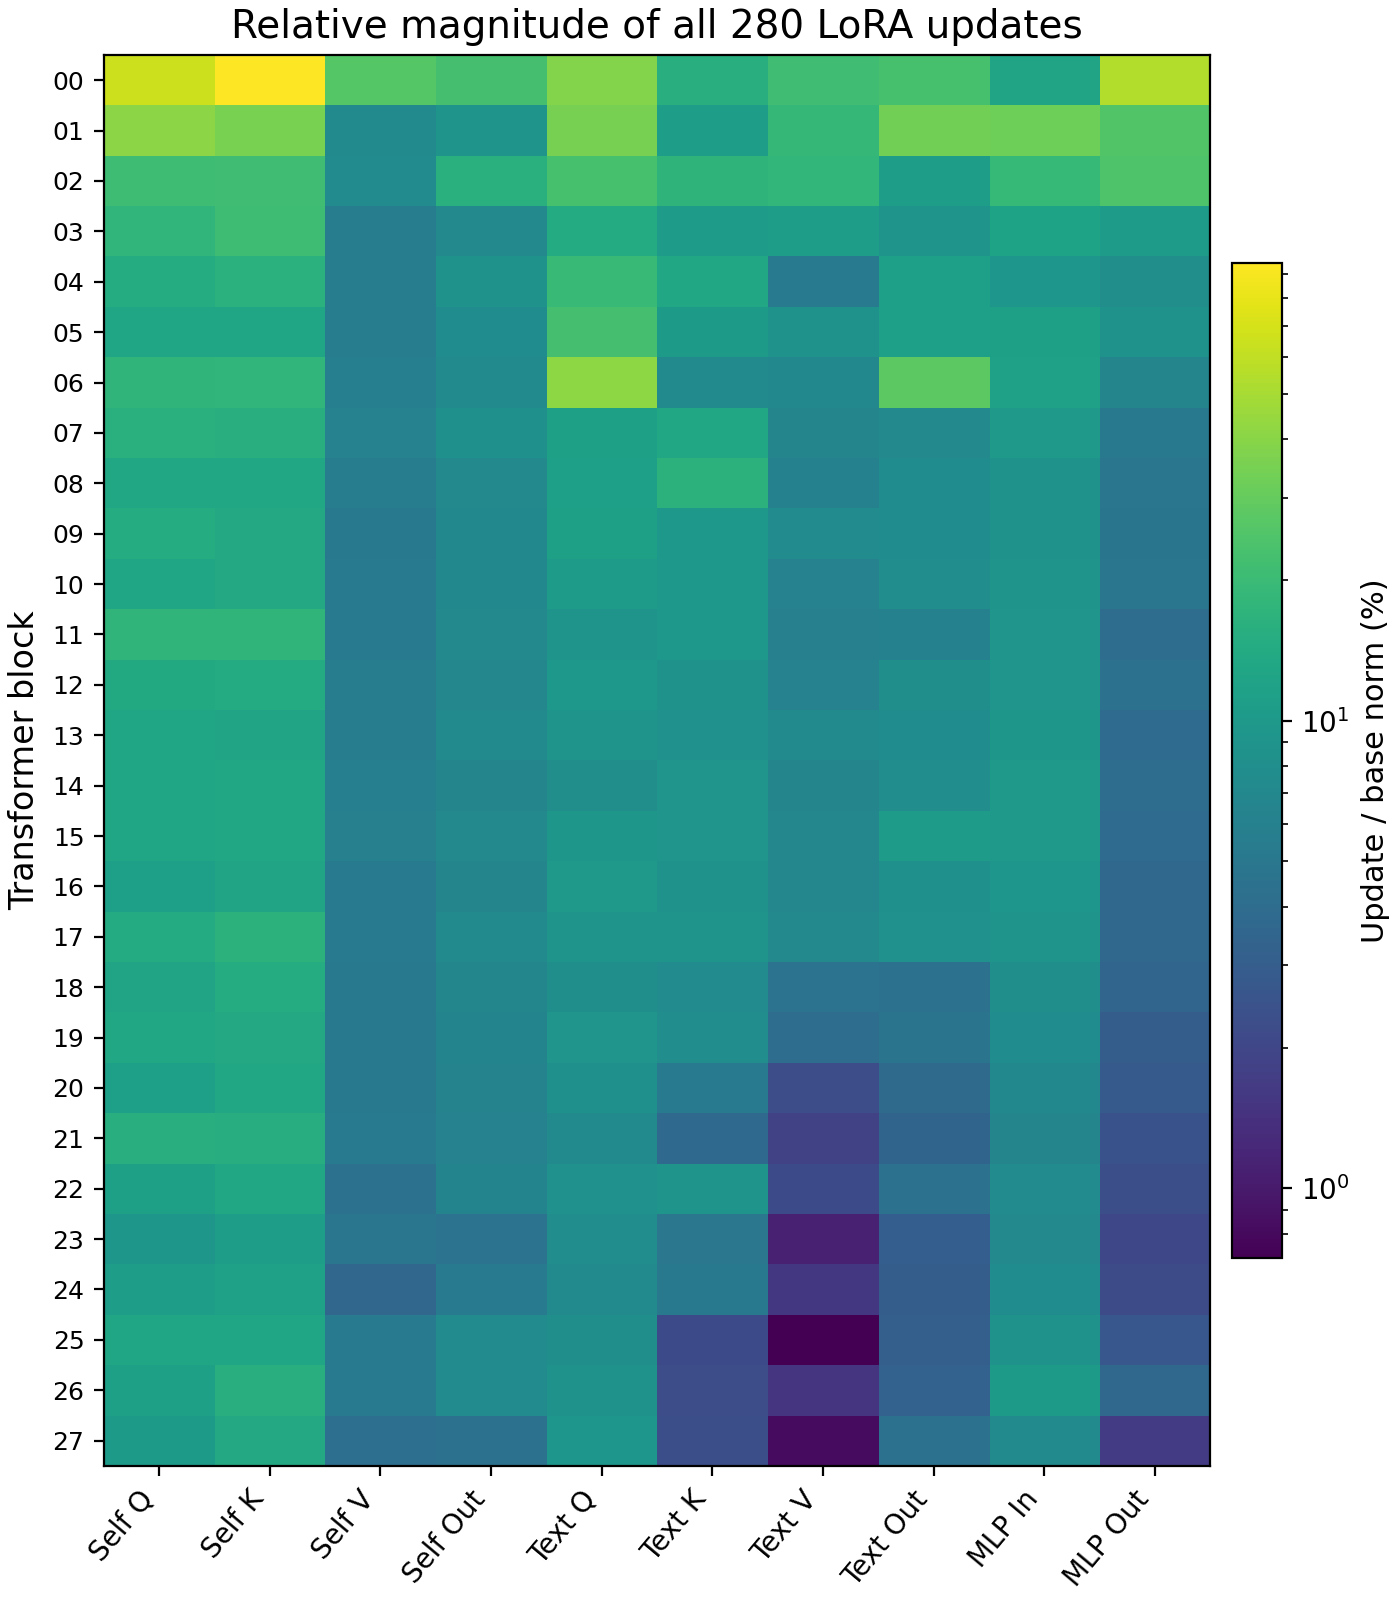
\includegraphics[width=0.9\textwidth]{figures/lora_updates_full.png}
\caption{Update-norm ratios $\lVert\Delta W\rVert_F/\lVert W\rVert_F$ for all 280 adapted projections across 28 blocks. The color scale is logarithmic.}
\label{fig:full-distributions}
\end{figure*}

\begin{figure*}[t]
\centering
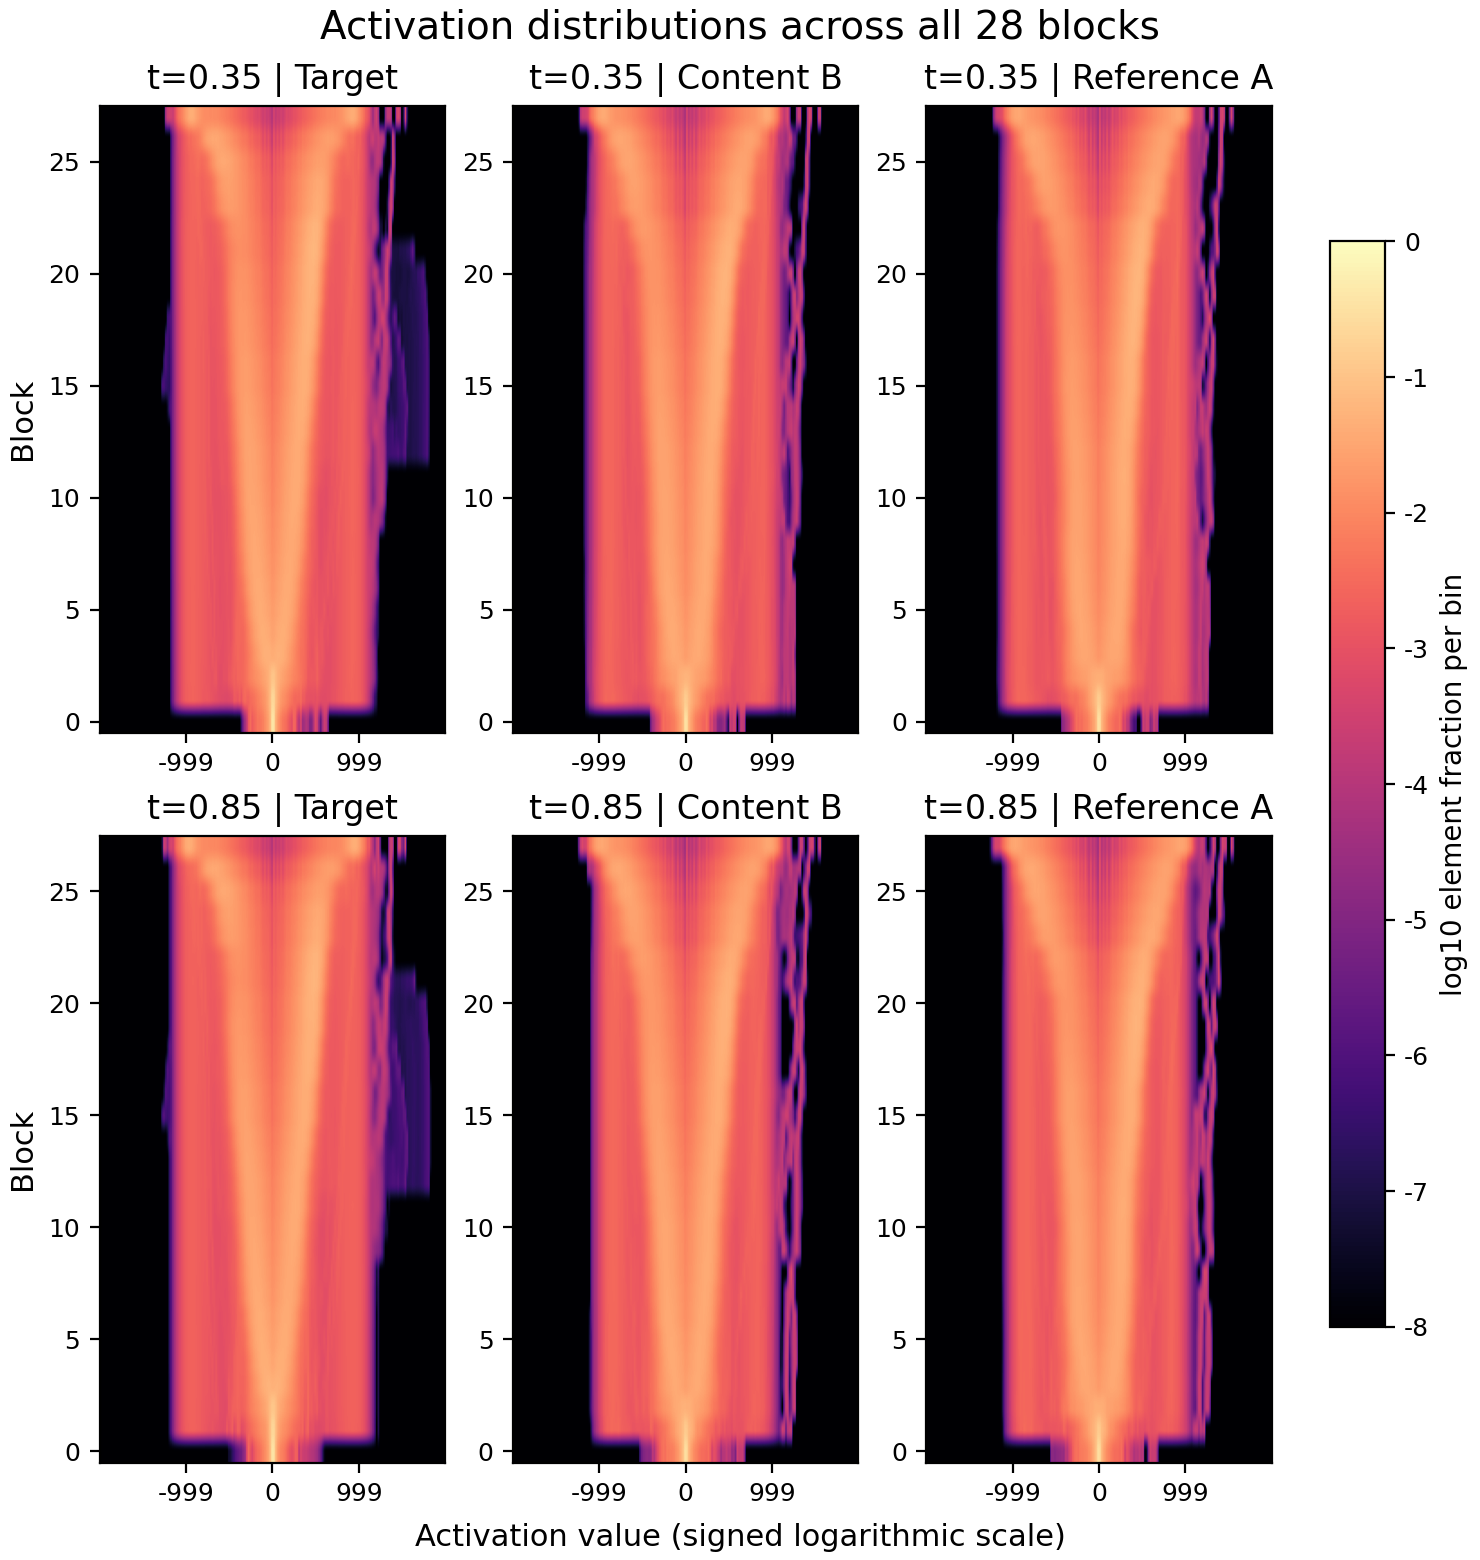
\includegraphics[width=0.9\textwidth]{figures/activation_full.png}
\caption{Signed-log histograms for the target, $B$, and $A$ slots over 28 blocks at two noise times. Each panel aggregates 69 external active-LoRA conditions.}
\label{fig:activation-distributions}
\end{figure*}

\begin{figure*}[t]
\centering
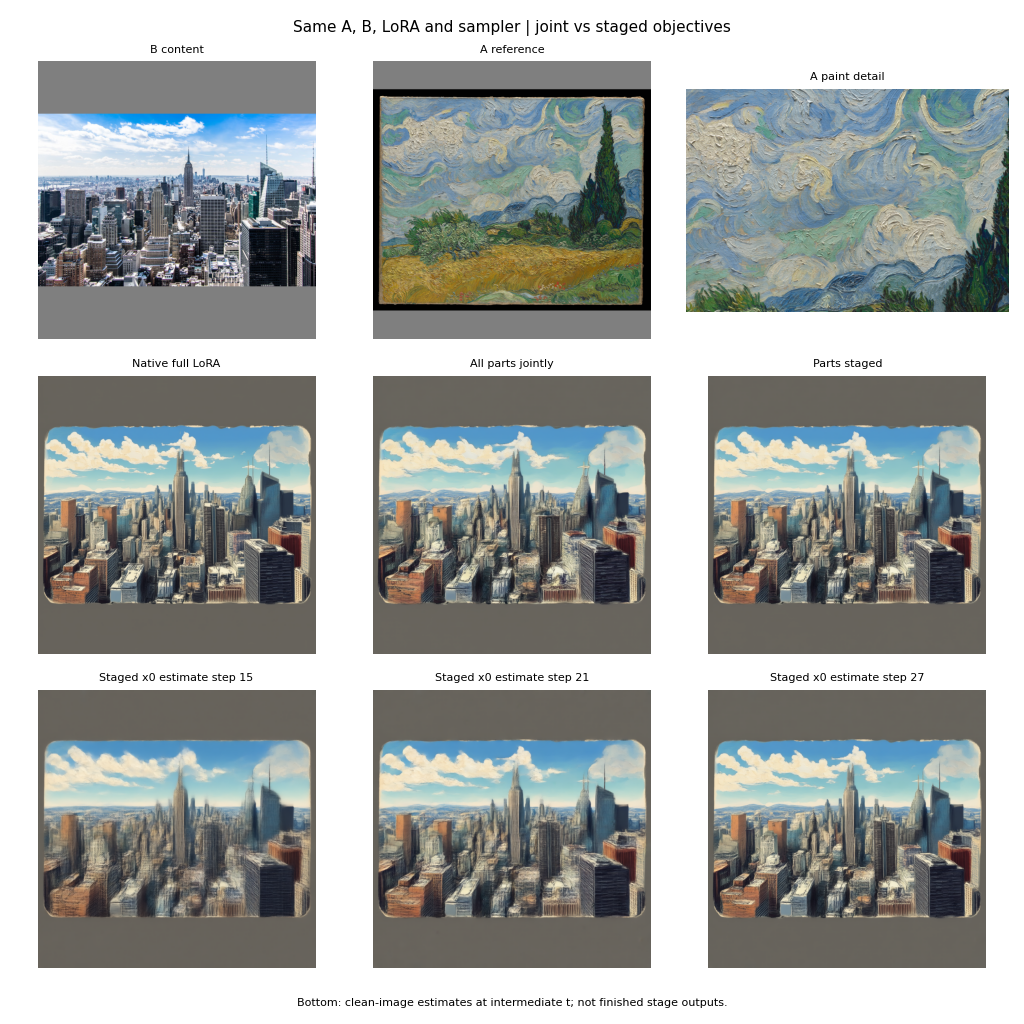
\includegraphics[width=0.9\textwidth]{figures/a_parts_comparison.png}
\caption{Reference-decomposition paths. Top row, left to right: content $B$, reference $A$, reference detail. Middle row: native, joint, staged outputs. Bottom row: VAE-decoded staged $\widehat z_0$ estimates at solver indices 15, 21, and 27; these are not completed intermediate outputs.}
\label{fig:parts-supplement}
\end{figure*}

\begin{figure*}[t]
\centering
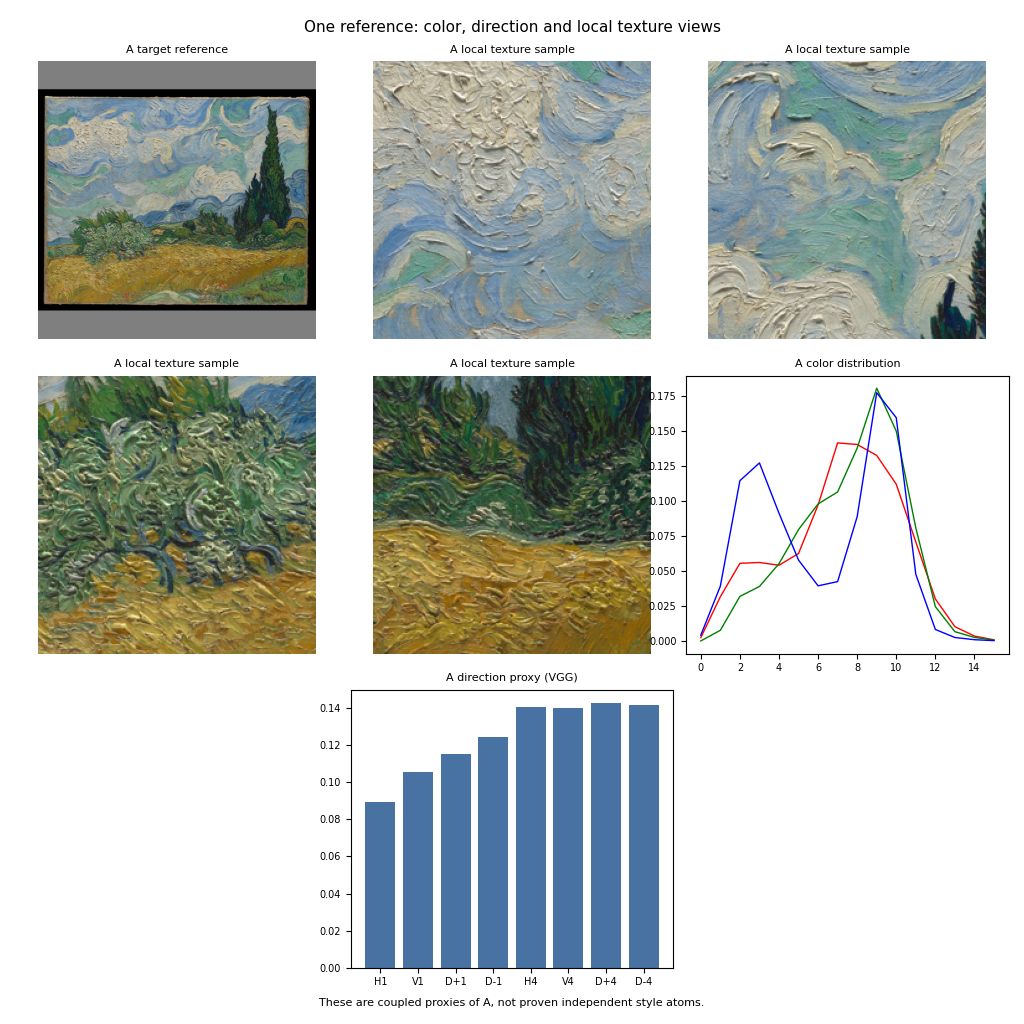
\includegraphics[width=0.9\textwidth]{figures/a_parts_reference.png}
\caption{Reference-derived targets. Top row: full reference and two local patches; middle row: two more patches and the RGB histogram; bottom: gray-VGG directional proxy. These coupled descriptors are not verified independent style atoms.}
\label{fig:parts-reference}
\end{figure*}

\end{document}
